\documentclass{myBeamer}

%%%%%%%%%%%%%%%%%%%%%%%%%
%% Header for standard beamer presentation
%%
%%  PresentationHeader.tex
%%
%%%%%%%%%%%%%%%%%%%%%%%%%

\documentclass[english,10pt]{beamer}



%%%%%%%%%%%%%%%%%%%%%%%%%%
%% TEMPLATES
%%%%%%%%%%%%%%%%%%%%%%%%%%


% Simple Tabular

%\begin{tabular}{ |c|c|c| } 
% \hline
% cell1 & cell2 & cell3 \\ 
% cell4 & cell5 & cell6 \\ 
% cell7 & cell8 & cell9 \\ 
% \hline
%\end{tabular}





%%%%%%%%%%%%%%%%%%%%%%%%%%
%% Packages
%%%%%%%%%%%%%%%%%%%%%%%%%%



% encoding 
\usepackage[utf8]{inputenc}
\usepackage[T1]{fontenc}


% general packages without options
\usepackage{amsmath,amssymb,amsthm,bbm}

% graphics
\usepackage{graphicx,transparent,eso-pic}

% text formatting
\usepackage[document]{ragged2e}
\usepackage{pagecolor,color}
%\usepackage{ulem}
\usepackage{soul}


% conditions
\usepackage{ifthen}





%%%%%%%%%%%%%%%%%%%%%%%%%%
%% Maths environment
%%%%%%%%%%%%%%%%%%%%%%%%%%

%\newtheorem{theorem}{Theorem}[section]
%\newtheorem{lemma}[theorem]{Lemma}
%\newtheorem{proposition}[theorem]{Proposition}
%\newtheorem{corollary}[theorem]{Corollary}

%\newenvironment{proof}[1][Proof]{\begin{trivlist}
%\item[\hskip \labelsep {\bfseries #1}]}{\end{trivlist}}
%\newenvironment{definition}[1][Definition]{\begin{trivlist}
%\item[\hskip \labelsep {\bfseries #1}]}{\end{trivlist}}
%\newenvironment{example}[1][Example]{\begin{trivlist}
%\item[\hskip \labelsep {\bfseries #1}]}{\end{trivlist}}
%\newenvironment{remark}[1][Remark]{\begin{trivlist}
%\item[\hskip \labelsep {\bfseries #1}]}{\end{trivlist}}

%\newcommand{\qed}{\nobreak \ifvmode \relax \else
%      \ifdim\lastskip<1.5em \hskip-\lastskip
%      \hskip1.5em plus0em minus0.5em \fi \nobreak
%      \vrule height0.75em width0.5em depth0.25em\fi}


%%%%%%%%%%%%%%%%%%%%
%% Idem general commands
%%%%%%%%%%%%%%%%%%%%

%% Commands

\newcommand{\noun}[1]{\textsc{#1}}


%% Math

% Operators
\DeclareMathOperator{\Cov}{Cov}
\DeclareMathOperator{\Var}{Var}
\DeclareMathOperator{\E}{\mathbb{E}}
\DeclareMathOperator{\Proba}{\mathbb{P}}

\newcommand{\Covb}[2]{\ensuremath{\Cov\!\left[#1,#2\right]}}
\newcommand{\Eb}[1]{\ensuremath{\E\!\left[#1\right]}}
\newcommand{\Pb}[1]{\ensuremath{\Proba\!\left[#1\right]}}
\newcommand{\Varb}[1]{\ensuremath{\Var\!\left[#1\right]}}

% norm
\newcommand{\norm}[1]{\left\lVert #1 \right\rVert}



% argmin
\DeclareMathOperator*{\argmin}{\arg\!\min}



%% graphics

% renew graphics command for relative path providment only ?
%\renewcommand{\includegraphics[]{}}




\usetheme{Warsaw}

\setbeamertemplate{footline}[text line]{}
\setbeamercolor{structure}{fg=purple!50!blue, bg=purple!50!blue}

\setbeamercovered{transparent}

\setbeamertemplate{footline}[frame number]
\setbeamertemplate{navigation symbols}{}


% shortened command for a justified frame
%\newcommand{\jframe}[2]{\frame{\frametitle{#1}\justify{#2}}}


%\newcommand{\jitem}[1]{\item \begin{justify} #1 \end{justify} \vfill{}}
\newcommand{\sframe}[2]{\frame{\frametitle{#1} #2}}



\newcommand{\indep}{\rotatebox[origin=c]{90}{$\models$}}



\usepackage{tikz}

\usepackage{multirow}


\usepackage{mdframed}

% in the case of ps graphics : convert ps to pdf
%\usepackage[usenames,dvipsnames]{pstricks}
%\usepackage{auto-pst-pdf}


%\usepackage[dvipsnames]{xcolor}
\usepackage{xcolor}


\makeatother



%%%%%%%%%%%%%%%%%%%%%
%% Begin doc
%%%%%%%%%%%%%%%%%%%%%

\begin{document}
\usepackage{csquotes}
\usepackage{pifont}
%\newcommand{\cmark}{\textcolor{green}\ding{51}}
%\newcommand{\xmark}{\textcolor{red}\ding{55}}
\newcommand{\cmark}{\ding{51}}
\newcommand{\xmark}{\ding{55}}

\title[Model validation]{Validation levels and standards depending on models types and functions}

\author{\noun{J. Raimbault}$^{1,2,3,\ast}$}

\institute{
$^1$ CASA, UCL\\
$^2$ UPS CNRS 3611 ISC-PIF\\
$^3$ UMR CNRS 8504 G{\'e}ographie-cit{\'e}s\medskip\\
$^{\ast}$ juste.raimbault@polytechnique.edu\medskip\\

\includegraphics[scale=2]{figures/openmole.png}
}

\date{\footnotesize CCS 2019\\
Satellite SIMEXPLO\\
October 2nd, 2019}

\begin{document}


\begin{frame}[plain]
	\titlepage
\end{frame}



% keywords:	Internal/external validation, Synthetic data, Model validation

%Abstract:	This presentation proposes an overview of what can be considered as validation, depending on model type (simulation, analytical, hybrid, spatial) and model function.



%%%%%%%
%% Notes (AUM, ~ macarthur)

% - open question calib coupled model / submodels : role of coupling in validation
% - cross validation in machine learning - imbricated levels of validation ?
% - statistical significance / levels of exigence (cf les 5 sigma du Higgs boson) : disciplinary standard ; 
% - depend also on knowledge domains? - we talk only about models here ? not really indeed ; model valid <=> theory valid ; empirical stylized facts ; validated datasets. An integrated view of validation ?
% - precise metrics ; standard protocols depend on the community
% - Postulate: validation linked to the function and/or the aim of the perspective ?
% - Validation % disciplines ? % models themselves ? "validated", "calibrated", "predictive" // knowledge domains. theory <-> modeling - integrates well into KD hypothesis ?
% - multiscale validation ? (cf horizontal/vertical matrix)
% - qualitative validation ?
% - pse : "beyond corroboration"

% - % model selection : multimodeling

% - POM: patterns 
% ( // generative social science)

% - Q of stochasticity: distribs

% - internal / external validation ; implementation (reproducible / language - indep etc) : computer science also different


\section{Introduction}

\sframe{(Un-)validated models?}{

% toy example of validations : schelling; model Wegener

\begin{columns}
	\begin{column}{0.5\textwidth}
		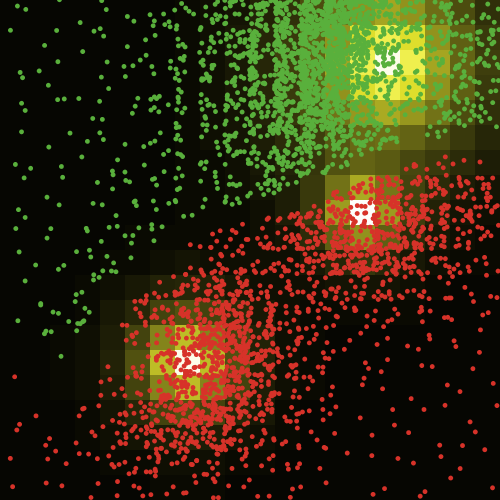
\includegraphics[width=\textwidth]{figures/schelling_ex0_t91.png}
		\medskip
		
		\textit{Schelling model (toy model)}
		
	\end{column}
	\begin{column}{0.5\textwidth}
		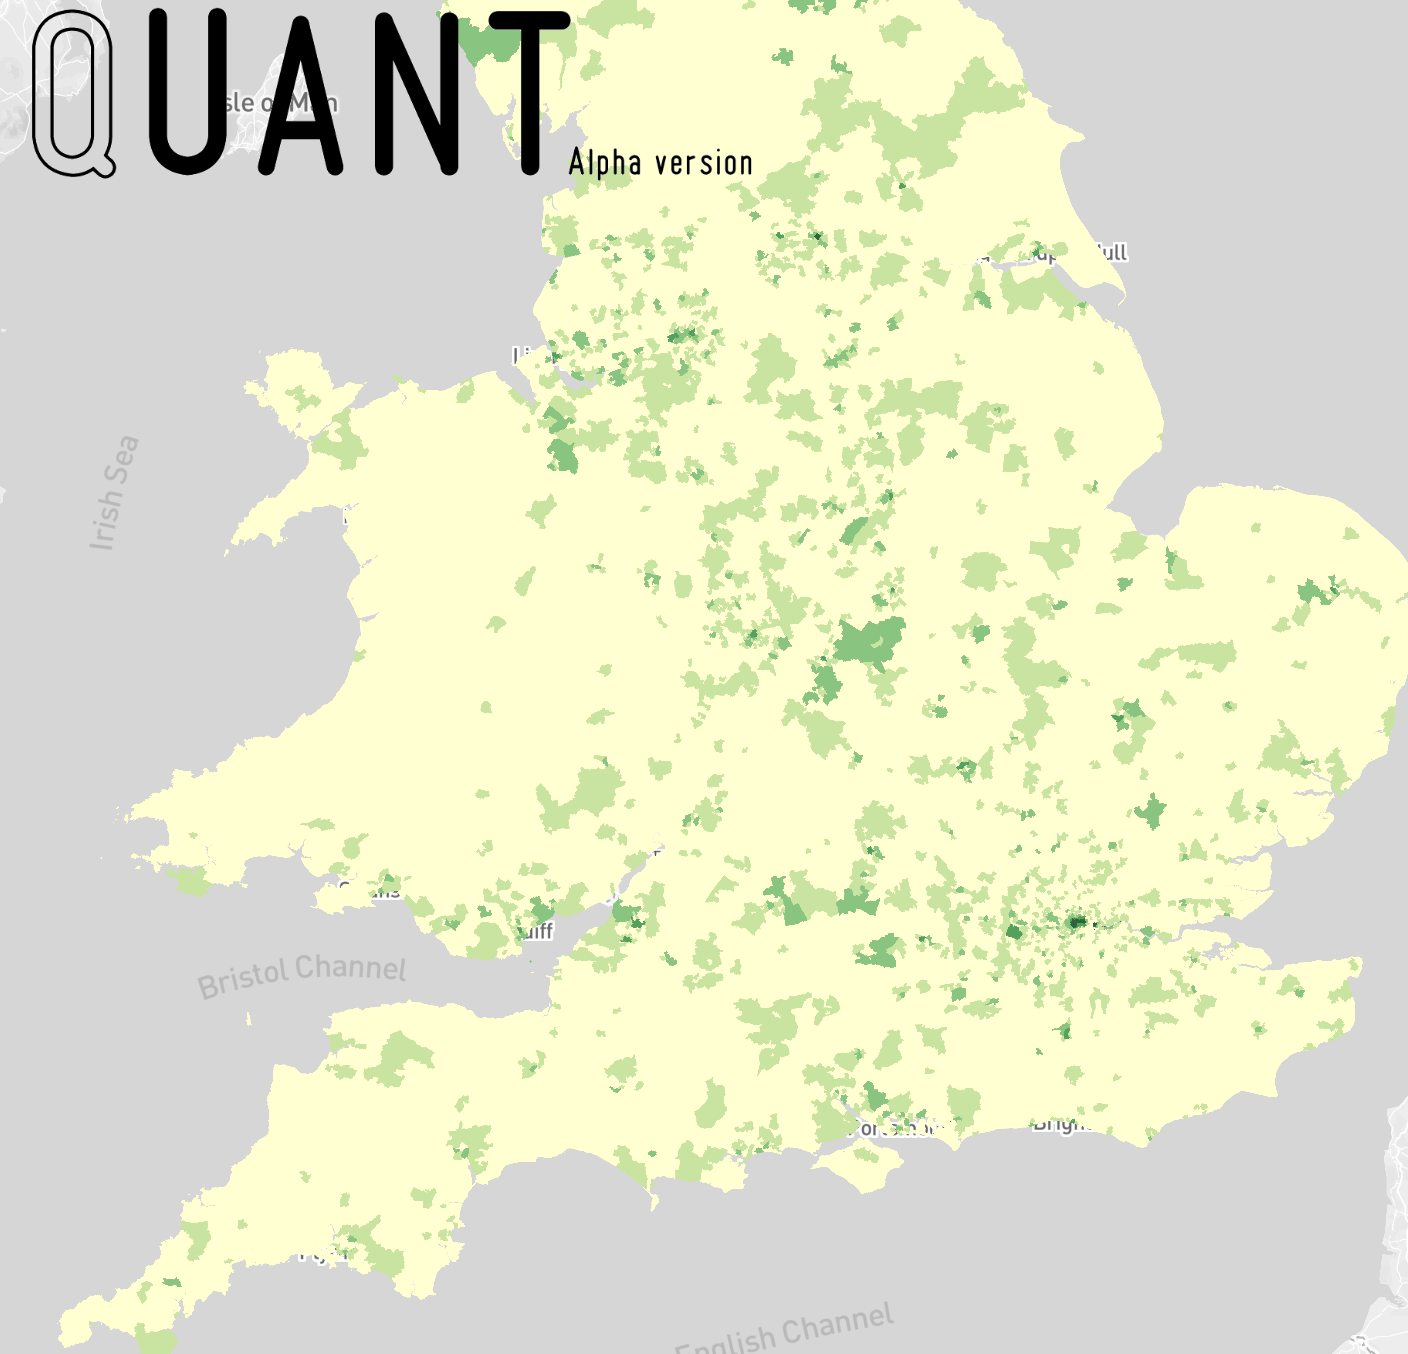
\includegraphics[width=\textwidth]{figures/quant.png}
		\medskip
		
		\textit{Quant model (operational models)}
		
	\end{column}
\end{columns}



}


\sframe{Model validation}{

% general def ?

\textbf{Proposed definition: } \textit{increasing the confidence in a model to fit its purpose}

\bigskip

Depends on:
\begin{itemize}
	\item model nature/type
	\item model purpose	
	\item discipline
	\item particular problem or application case
	\item expected standards %(e.g. embedded navigation systems)
	\item background or mood (!) of the reviewer/reader/listener
	\item \ldots
\end{itemize}


}

\sframe{Model validation}{

% \cite{barlas1990philosophical} philosophical roots of model validation. (for systems dynamics models). Causal/non-causal nature of models. Holistic-social-relativist VS reduciotnist/foundationalist => objective procedure vs conversational, continuum of usefulness

% + "social validation" = disciplinary integration / number of citations etc. (relates to different scientific practices)

\justify

$\rightarrow$ Validation has very different implications depending on epistemological positioning: from an objective procedure (reductionism) to a more conversational and reflexive process (holistic)

\cite{barlas1990philosophical}

\bigskip


$\rightarrow$ How disciplines are positioned, political relations, effective citation practices, etc. are all aspects of implicit ``social'' model validation

}


\section{Examples}

\sframe{Predictive models}{

%hydrology \cite{legates1999evaluating} quantitative agreement between model and data $\rightarrow$ numerous choice of indiccators - "robust" ones ? : validation of indicator choice itself ?
%meteo idem / geosci

In geosciences (hydrology e.g. \cite{legates1999evaluating}), quantitative agreement between model and data

\bigskip

$\rightarrow$ choice among numerous indicators to quantify the agreement

\medskip

$\rightarrow$ robust indicators? choice can be validated itself



% \cite{van2016review} Land-change modeling: particularity of spatial systems ?  Location accuracy assessed 68% Pattern accuracy assessed 23% Independent validation 37% Accounts for near hits 25% Reference model included 30% Uncertainty analysis conducted 17% Sensitivity analysis conducted 12% Validation not reported 31%

\bigskip

In practice, not systematically done, as for example for land-use change models \cite{van2016review}


% \cite{park2003microscopic}
% VISSIM model (traffic mmicrosimulation)  measure of effectiveness selection, (b) data collection, (c) calibration parameter identification, (d) experimental design, (e) run simulation, ( f ) surface function development, (g) candidate parameter set generations, (h) evaluation, and (i) validation through new data collection

\bigskip

Microsimulation models enter a similar context (e.g. \cite{park2003microscopic} for the Vissim traffic model), in a slightly different way than agent-based models

}


\sframe{Statistical models}{

%statistics: predictive power / error of different types

% \cite{hjorth2017computer} statistical models validation 

Statistical models exhibit different measures of ``model quality'':

\begin{itemize}
	\item predictive power (explained variance)
	\item p-value (alpha errors) and beta power (false positives)
\end{itemize}


\bigskip

% \cite{saltelli2019short}
%. - danger of modeling hubris and transscience (responses in domains scicne cannot)
%  - should be inspired from structure and standards from statistics
%  - eexternal auditing 
%. - ethics of quantification
%. - reflexive approach ! (links to complexities chapter !) - post normal science

Following \cite{saltelli2019short}, mathematical modeling may benefit similar standards as in statistics


}


\sframe{Analytical models}{

% kind of tricky as would be more linked to the discipline ?

\justify

$\rightarrow$ to what extent of analytical resolution is a model ``validated''? (limit theorem, restricting assumptions, unfeasible ranges in practice, \ldots)

\medskip

$\rightarrow$ finally most of the time coupled with numerical simulation? see coupling of machine learning and mathematical modeling

\cite{butler2018machine} or statistical inference \cite{bzdok2018points}

\medskip

$\rightarrow$ computational turn of science \cite{arthur2013complexity}?

\bigskip

\textit{On the link with simulation models:}

\medskip

\begin{itemize}
	\item Formal proof systems remain limited
	\item Undecidability of the Turing machine Halting problem	
\end{itemize}


}



\sframe{Simulation models}{

% \cite{sargent2010verification} (more recent) : "independant validation and verification" (sci as cognitive agents) ; can be interactive with model development ; scoring model of the model . Problem entity (system) / computerized model / conceptual model : not too far from knowledge domains. Iterative process.
% Validation techniques: Animation, Comparison to Other Models, Degenerate Tests, Event Validity, Extreme Condition Tests, Face Validity, Historical Data Validation, Historical Methods, Internal Validity, Multistage Validation, Operational Graphics (run behavior), vParameter Variability - Sensitivity Analysis, Predictive Validation, Traces (follow model entitites), Turing Tests : ! cf Fake Life context ALife
% Operational validity: range of methods : explore behavior, comparison of outputs, graphical compairons, confidence intervals, hypothesios test, 
% Documentation of model validation is crucial ! (convince user in a sense)
% recommentded procedure : for operational models.
% Accreditation (ex US DoD)



Overview of simulation model validation methods and processes by \cite{sargent2010verification}

\medskip

\begin{enumerate}
	\item independent validation and verification (modelers as cognitive agents \cite{giere2010explaining}
	\item iterative process between conceptual, computerized models, and the system itself
	\item Numerous validation techniques: comparison, extreme conditions, historical data, internal validity, sensitivity analysis, predictive performance, Turing test
	\item Specific techniques for operational validity
	\item Documentation of the validation process is crucial
	\item Accreditation: science as a social process
\end{enumerate}

\medskip

% \cite{landry1983model} ~ old paper in RO; still relevant: confidence, credibility and reliability, model assessment and evaluation, usefulness and usability of the model ; 
% - conceptual validation ; logical validation ; experimental validation ; operational validation ; data validation 

\cite{landry1983model} similar in operations research



% \cite{balci1994principles} simulation model validation : 15 principles : ??? (no full text)


}



\sframe{Simulation models as generative models}{

Simulating the evolution of a system in a generative way:

\cite{epstein1996growing}: ``\textit{if you did not grow it, you did not explained it}''

\medskip

$\rightarrow$ similar to \textit{Pattern Oriented Modeling} \cite{grimm2005pattern}: reconstruct (macro) patterns from the bottom-up

\medskip

Implications for validation:
\begin{itemize}
	\item Crucial role of indicator choice (see e.g. link prediction vs. network structure reconstruction)
	\item fine understanding of model behavior
	\item role of processes and parameters
	\item controlled experiments (\textit{virtual laboratories})	
\end{itemize}

\medskip

$\rightarrow$ typical example of \textbf{explication/comprehension} models (but which can also be statistical, analytical)

% rq : instrumental vriabels models are also explicative? analytical can also be

}




\sframe{Sensitivity analysis}{

% \cite{saltelli2010variance} sensitivity indices - part of model validation.

% \cite{cariboni2007role} the role of sensitivity analysis in ecological modeling : best practices - refined methodological tree.

\justify

$\rightarrow$ Sensitivity analysis is part of a model validation process 

\cite{saltelli2010variance}: how does a model behave in response to variations in its parameters/variables/input data?

\bigskip

$\rightarrow$ Articulation of complementary methods \cite{cariboni2007role} (validation is then the full cascade of successive methods applied)


}




\sframe{Sensitivity analysis: examples of properties}{

%\textit{Properties of different sensitivity analysis techniques}

% rq : as always, choice of method to validate related to its properties, the question asked, etc.

\textbf{\textit{Design of Experiments}}


\begin{mdframed}

\begin{columns}
	\begin{column}{0.2\linewidth}
	
	\bigskip
	\bigskip
	
	One factor at a time
	
	\medskip
	
	Complete plan
	
	\medskip
	
	LHS/Sobol
		
	\end{column}
	\begin{column}{0.2\linewidth}
		
		\textbf{Coverage}
		
		\bigskip
		
		{\textcolor{red}
		\xmark
		}
		
		\medskip
		
		{\textcolor{green}
		\cmark
		}
		
		\medskip
		
		{\textcolor{green}
		\cmark
		}
			
	\end{column}
	
	\begin{column}{0.25\linewidth}
		
		\textbf{Interpretability}
		
		\bigskip
		
		{\textcolor{green}
		\cmark
		}
		
		\medskip
		
		{\textcolor{green}
		\cmark
		}
		
		\medskip
		
		{\textcolor{red}
		\xmark
		}	
	\end{column}
	
	\begin{column}{0.2\linewidth}
		
		\textbf{Budget}
		
		\bigskip
		
		{\textcolor{green}
		\cmark
		}
		
		\medskip
		
		{\textcolor{red}
		\xmark
		}
		
		\medskip
		
		{\textcolor{green}
		\cmark
		}	
	\end{column}

	
	
	
\end{columns}

	
\end{mdframed}

\bigskip

\textbf{\textit{Sensitivity analysis}}

\begin{mdframed}
	\begin{columns}
	\begin{column}{0.2\linewidth}
	
	\bigskip
	\bigskip
	
	Morris
	
	\medskip
	
	Saltelli
	

		
	\end{column}
	\begin{column}{0.2\linewidth}
		
		\textbf{Coverage}
		
		\bigskip
		
		{\textcolor{red}
		\xmark
		}
		
		\medskip
		
		{\textcolor{green}
		\cmark
		}
		
	
			
	\end{column}
	
	\begin{column}{0.25\linewidth}
		
		\textbf{Interpretability}
		
		\bigskip
		
		{\textcolor{green}
		\cmark
		}
		
		\medskip
		
		{\textcolor{green}
		\cmark
		}
			
	\end{column}
	
	\begin{column}{0.2\linewidth}
		
		\textbf{Budget}
		
		\bigskip
		
		{\textcolor{green}
		\cmark
		}
		
		\medskip
		
		{\textcolor{red}
		\xmark
		}
			
	\end{column}

	
	
	
\end{columns}
	
\end{mdframed}



}




\sframe{Exploration of simulation models}{

\justify

\textbf{Model exploration} is running a simulation model, following a \emph{design of experiments}, to gain knowledge about \emph{model properties}.

\medskip

e.g. : sensitivity analysis 

\bigskip

Recent and significant increase in the development of methods to explore, calibrate and optimize (geo)simulation models.
%
\bigskip

$\rightarrow$ part of model validation also

\bigskip

\textbf{Explicative / comprehensive models} are mostly made useful by their exploration

}


%
\sframe{Advanced exploration methods}{

Example of validation methods included in OpenMOLE:

\textbf{Calibration}: Evolutionary (GA) and Bayesian (ABC) methods 

\bigskip

\textbf{Diversity Search}: unveil the variety of obtainable patterns in output space: can the model produce unexpected patterns, and if so what does it means for its mechanisms ?

\bigskip

\textbf{Origin Search}: inverse problem, tackling the problem of equifinality

}



\sframe{New methods: spatial sensitivity}{

\textit{Spatial sensitivity analysis techniques}


\bigskip

Example: generators of synthetic urban districts \cite{doi:10.1162isal_a_00159}

\medskip

\centering

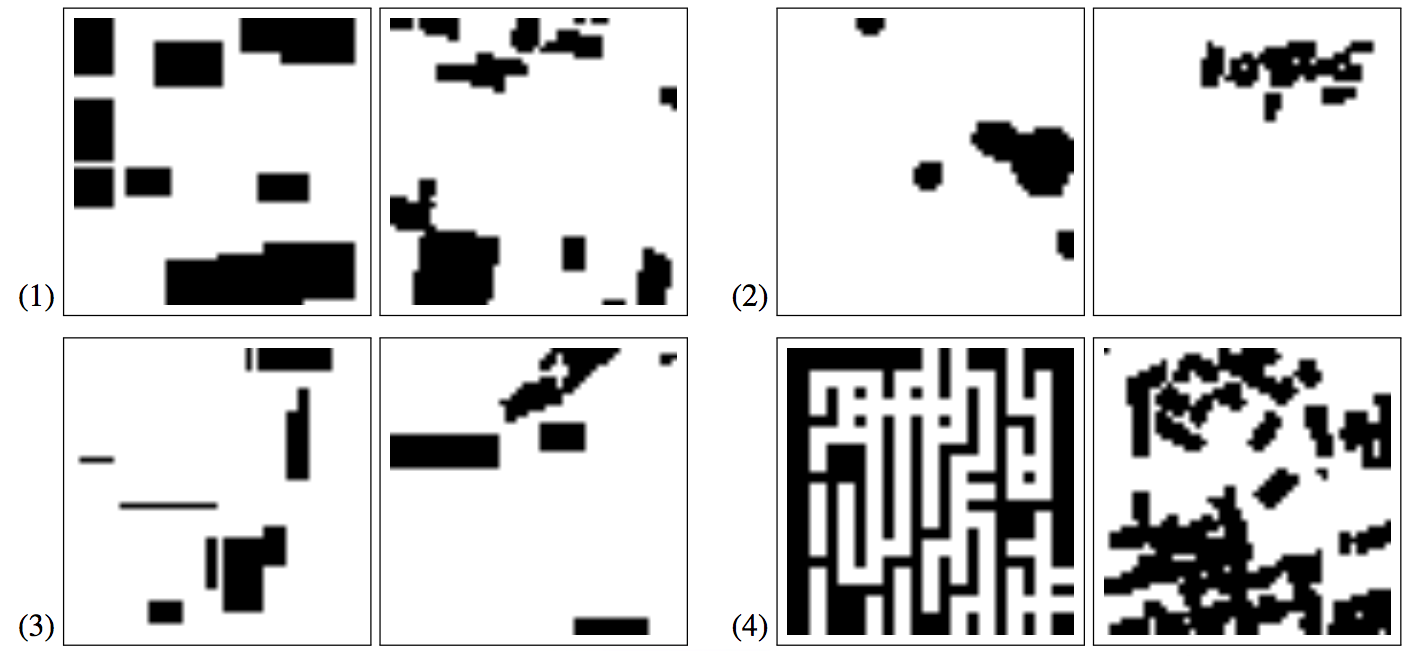
\includegraphics[width=\textwidth]{figures/spatialsens_calib.png}

}



\sframe{Multi-modeling}{


%% - importance of multi-modeling / model comparison / model coupling


$\rightarrow$ Validation of submodels to foster diverse questions and approaches


\medskip

$\rightarrow$ Validation of coupled models remains an open question (e.g. error propagation techniques)


\medskip

$\rightarrow$ Comparison of the model with alternative formalisms: for example agent-based modeling against differential equations

\medskip

$\rightarrow$ Importance of systematic model benchmarks/classifications

}



\section{Classifications}

\sframe{Validation and model functions}{

% roughly correspondance function <-> type of validation

Varenne's model function families \cite{varenne2017theories}:

\medskip

\begin{itemize}
	\item \textbf{Perception and observation}: perception medium, visualization, experimental medium
	\item \textbf{Understanding}: description, prediction, explication, comprehension
	\item \textbf{Theory construction}: interpretation of a theory, test of internal coherence, applicability, co-computability
	\item \textbf{Communication}: scientific communication, stakeholders involvement
	\item \textbf{Decision-making}: planning, decision-making, self-fulfilling system prescription
\end{itemize}
 
 % the last : finance but also smart cities

% comprehension more general than explication: assumes projection/reconstruction of system structure within the psychological structure considering it. explanation: reconstruction of causal chains.

}

\sframe{Validation and model functions}{

\begin{itemize}
	\item \textbf{Perception and observation}: how much information is extracted
	\item \textbf{Description}: how much information is contained within
	\item \textbf{Prediction}: predictive power (quantitative indicators or qualitative behavior)
	\item \textbf{Explication and comprehension}: how much of the causal structure of the system is grasped
	\item \textbf{Theory construction}: how does the model contributes to the theory, to coupling of its components (e.g. medium for interdisciplinarity)
	\item \textbf{Communication}: how much information is conveyed and to which agents
	\item \textbf{Decision-making}: how are decision supported, which benefits and for what dimension (societal, environmental, etc.)?
\end{itemize}

}


\sframe{Validation and model type}{

% idem with model type

\begin{itemize}
	\item \textbf{Statistical}: model fit/statistical power
	\item \textbf{Machine learning}: predictive power
	\item \textbf{Analytical}: level of resolution, genericity
	\item \textbf{Simulation/generative}: model behavior, sensitivity analysis, pattern reconstruction, causal processes
	\item \textbf{Operational}: planning/decision-making relevance
	\item \ldots
\end{itemize}

\medskip

\textit{Rq: classification of ``model types'' can neither be exhaustive nor consistent}


}



\sframe{Social aspects of validation}{

\begin{itemize}
	\item Acceptance and impact within the discipline/specific subject of study
	\item Impact in other disciplines
	\item Impact outside of science
	\item Interdisciplinary/bridging/integrative role \cite{raimbault2019exploration}
	\item Different dimensions: complex and multidimensional nature of scientometrics \cite{raimbault2019exploration} \cite{cronin2014beyond}
	\item \ldots
\end{itemize}


}



\section{Discussion}


\sframe{Validation within a knowledge framework}{

\justify

Epistemological foundations of a knowledge framework for integrated approaches to complex systems \cite{raimbault2017applied}, coined by 

\cite{raimbault2019exploration} as \textbf{Applied Perspectivism}:

\bigskip

Giere's cognitive approach to science~\cite{giere2010explaining} : cognitive agents have \textit{perspectives} on aspects of the real world.

\bigskip

\textbf{Scientific perspectivism} \cite{giere2010scientific} : \emph{cognitive agents} use \emph{media}, the models, to represent something with a certain purpose.

\bigskip

\cite{varenne2017theories}'s classification of main model functions : perception and observation, understanding, theory building, communication, decision making.


}


\sframe{Knowledge domains}{

\textit{Definition of Knowledge Domains : }

\begin{itemize}
\item \textbf{Empirical.} Empirical knowledge of real world objects.
\item \textbf{Theoretical.} Conceptual knowledge, implying cognitive constructions.
\item \textbf{Modeling.} The model as the formalized \emph{medium} of the perspective.
\item \textbf{Data.} Raw information that has been collected.
\item \textbf{Methods.} Generic structures of knowledge production.
\item \textbf{Tools.} Implementation of methods and supports of others domains. % Proto-methods
\end{itemize}

}


\sframe{Knowledge framework}{

\textbf{Description of the Knowledge Framework : }

\bigskip

\begin{enumerate}
	\item Any scientific knowledge construction on a complex system can be understood as a perspective, decomposed into knowledge domains.
	\item Contents within domains \textit{coevolve}~\cite{holland2012signals} between themselves and with other elements of the perspective (including cognitive agents and the purpose).
	\item It implies weak emergence~\cite{bedau2002downward} what is consistent with the existence of bodies of knowledge.
\end{enumerate}

}


\sframe{Interactions between domains}{

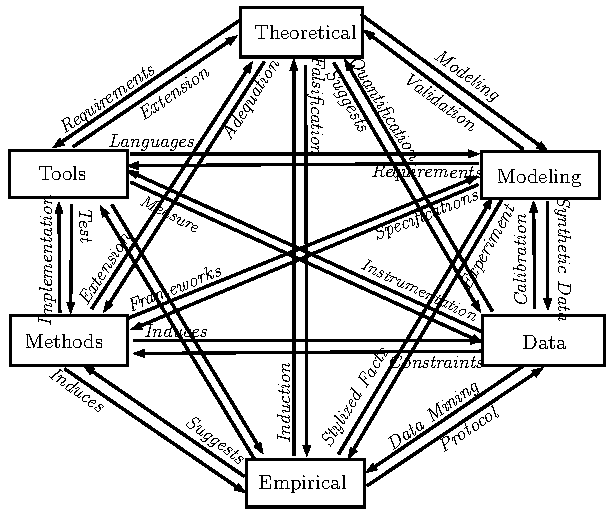
\includegraphics[height=0.9\textheight]{figures/framework.pdf}

}



\sframe{Validation within the knowledge framework}{

$\rightarrow$ Role and type/method of validation are proper to each perspective

\medskip

$\rightarrow$ Links and interaction between domains are part of the model/theory construction process and thus of validation of the perspective

\medskip

$\rightarrow$ Intrinsically iterative nature of validation

\medskip

$\rightarrow$ Cannot be dissociated (at least for the study of complex systems) to new methods and tools

}



\sframe{Conclusion}{

% conclusion and discussion

\justify

$\rightarrow$ Meaning of ``model validation'' is indeed strongly dependant on its properties, including type, function, context of application, discipline

\bigskip

$\rightarrow$ \textit{Obvious?} Not for all seeing some debates/questions here and there. \textbf{Interdisciplinarity requires an opening to other standards/definitions/viewpoints}

\bigskip

$\rightarrow$ Validation within the Applied Perspectivism knowledge framework: validation proper to each perspective and to the coupling of perspectives, intrinsically iterative

\bigskip

$\rightarrow$ Construction of integrative theories and models implies this multiple view of model validation and the variety of methods and tools, in particular in the case of simulation models

}








%\backupbegin


%%%%%%%%%%%%%%%%%%%%%
\begin{frame}[allowframebreaks]
\frametitle{References}
\bibliographystyle{apalike}
\bibliography{biblio}
\end{frame}
%%%%%%%%%%%%%%%%%%%%%%%%%%%%


%\backupend





\end{document}


